\chapter{Integrated Mobile Platform}
\label{cha:Platform}

\begin{figure}
\centering
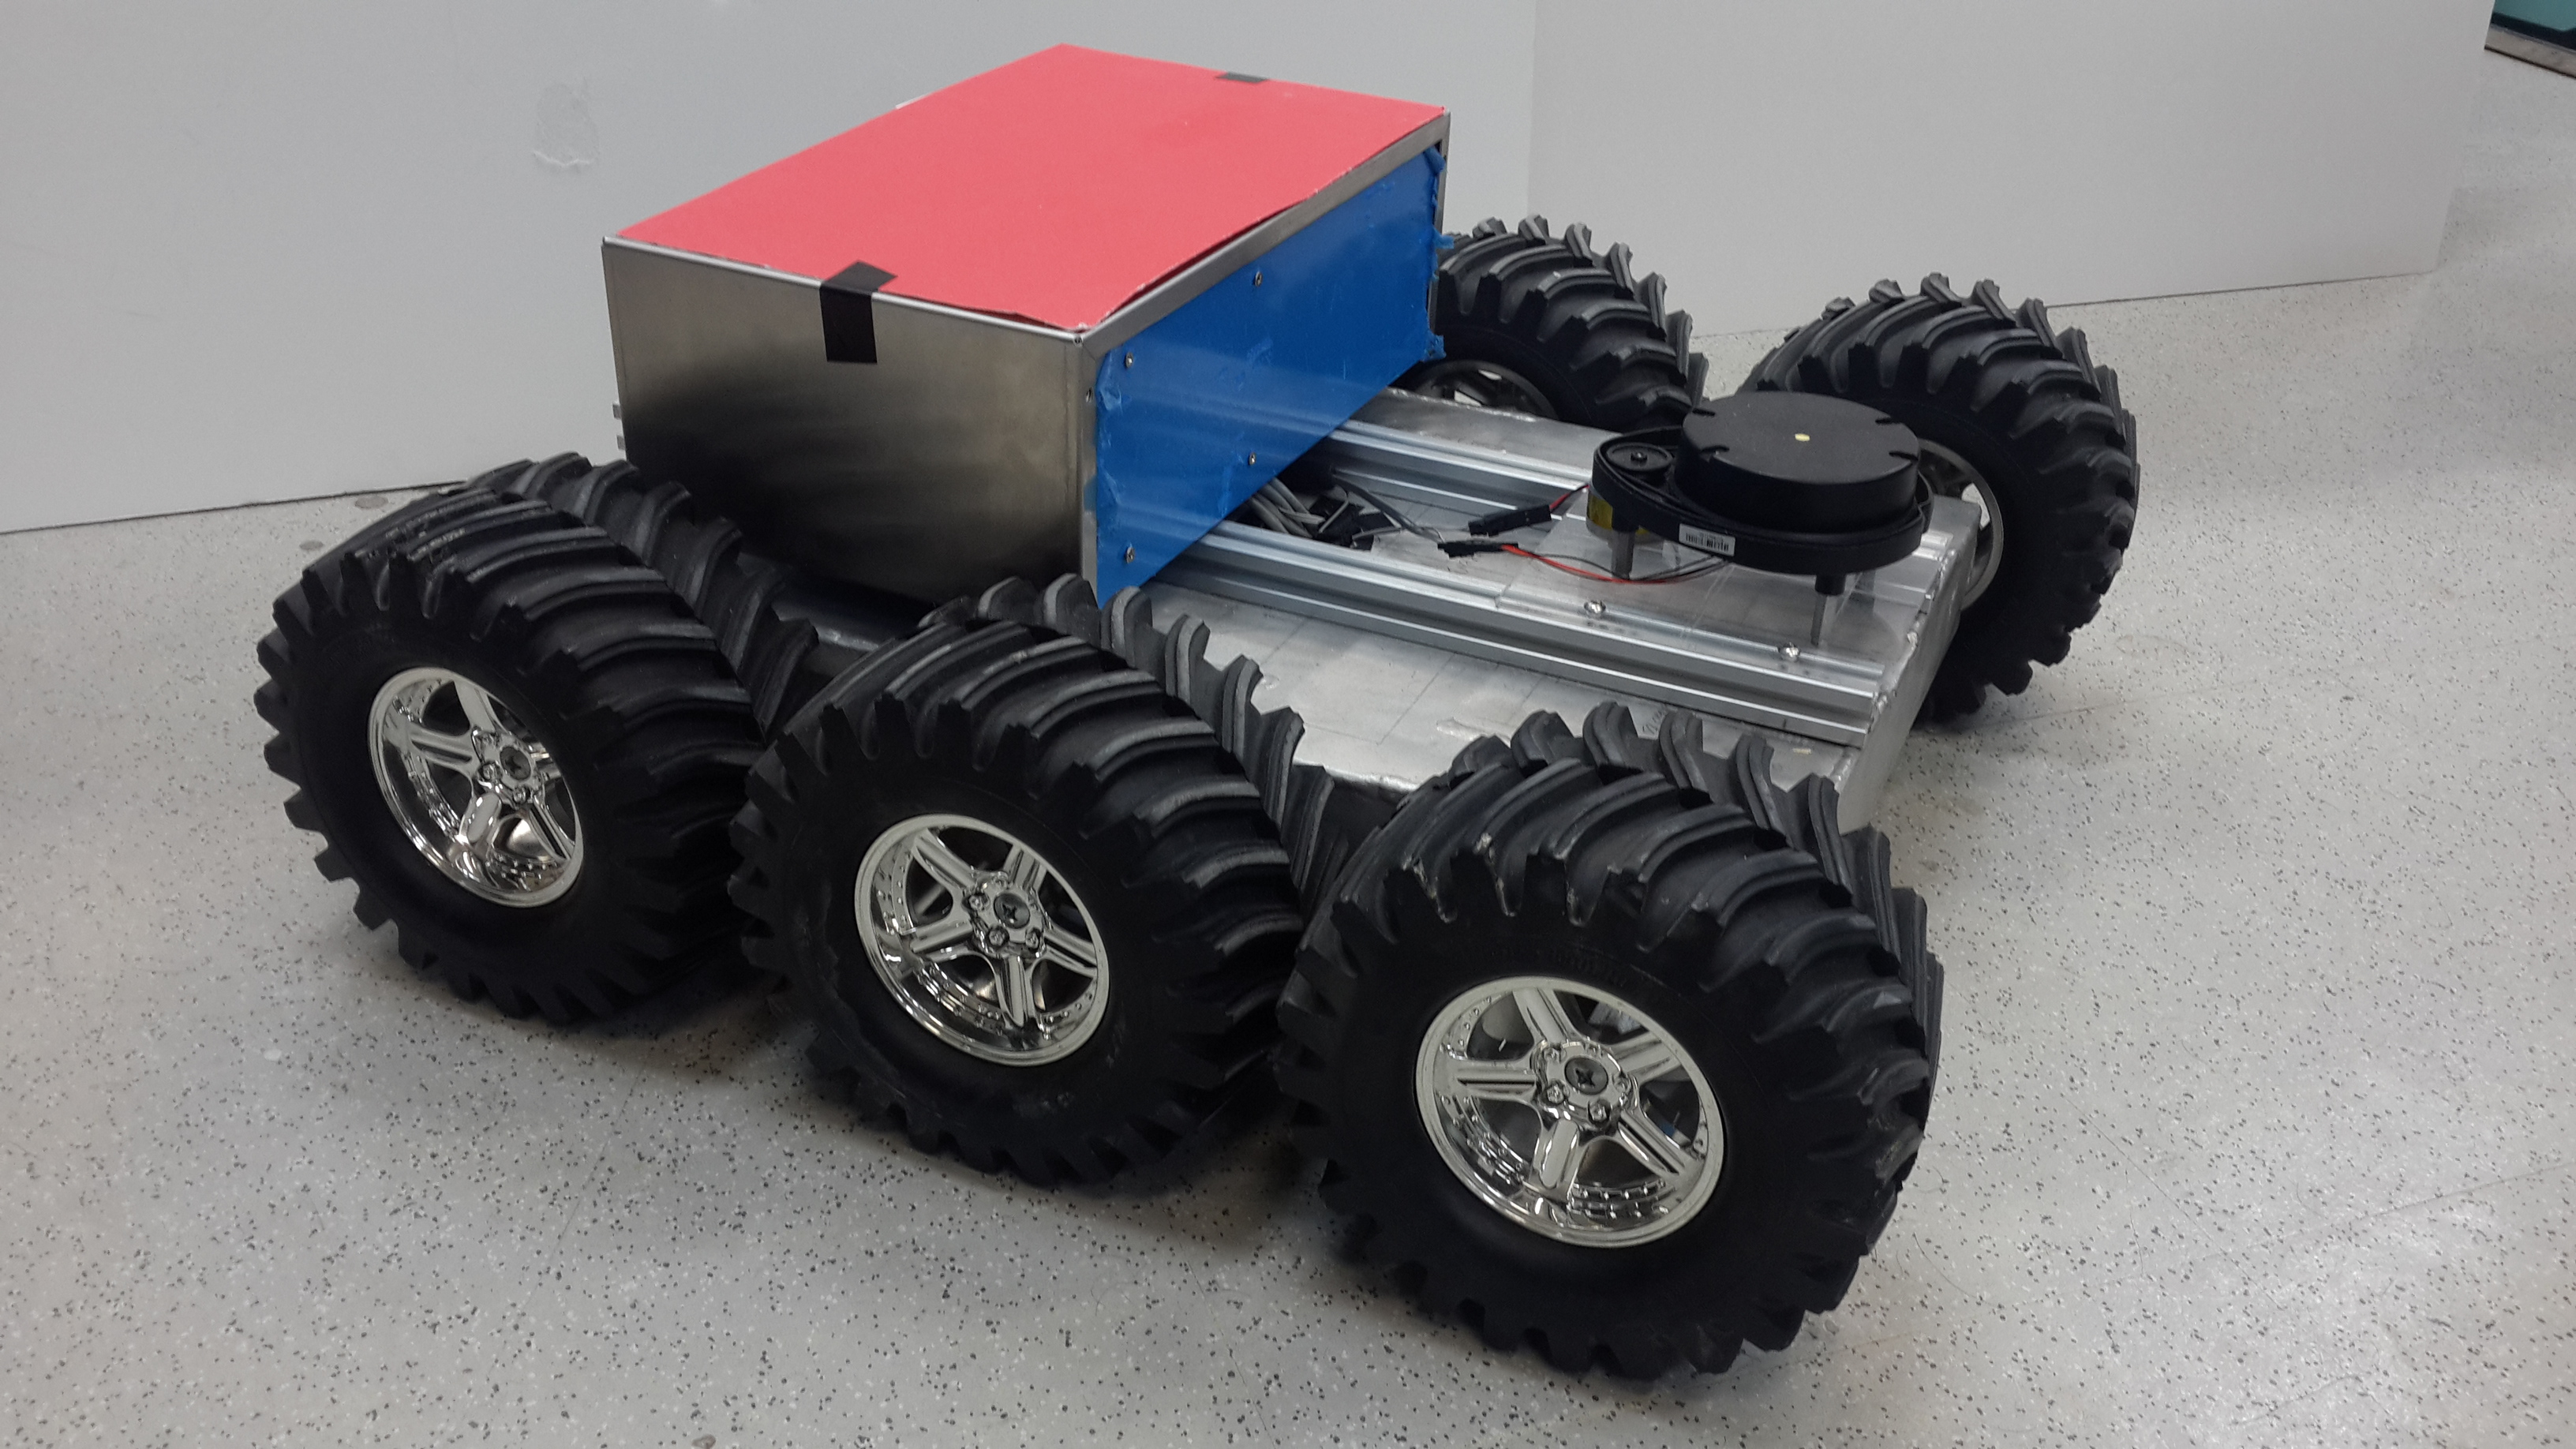
\includegraphics[width=0.5\textwidth]{IMP_color}
\caption{The Integrated Mobile Platform}
\end{figure}

\section{Overview}
\begin{figure}
\centering
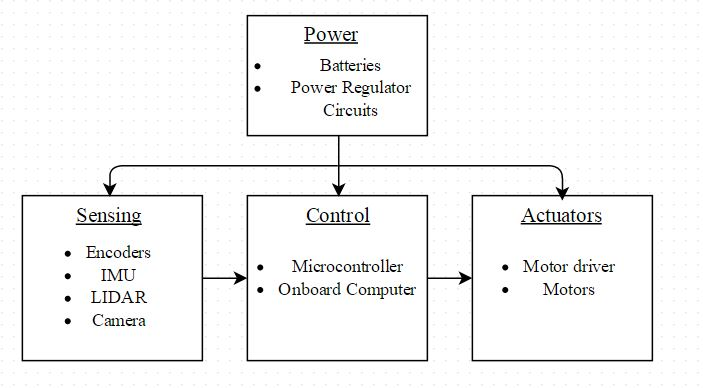
\includegraphics[width=0.8\textwidth]{blockDiag}
\caption{System diagram of the IMP}
\label{fig: blockDiag}
\end{figure}
The primary purpose of building the \imp or the IMP is to test the various algorithms that are used in SLAM. Since SLAM is mostly used for real time control, it is desirable to have platform with the capabilities to implement that. For this we need to keep the following considerations in mind. 
\begin{description}
	\item[Movement] Has to be able to move with a variety of speeds and relatively small turning radii as it is to be used indoors. 
	\item[Self-position acknowledgment] Has to have proprioceptive sensors which give an estimate of it's own position and orientation.
	\item[Environment sensing] Has to have sensors to understand the environment. 
	\item[On-board computer] Has to have sufficient on-board processing power to do the computations necessary for SLAM.
	\item[Real time controller] Has to have a capability to implement real time control.
	\item[Communication] Has to have robust communication between the different components and also with the ground station. 
	\item[Memory] Has to have sufficient on-board memory to collect data to enable testing of SLAM algorithms off line.  
	\item[Flexibility] The various components both hardware and software need to be designed in such a way that it is easy to switch them around.
\end{description}

In each stage these requirements act as guiding principles with emphasis given to the flexibility aspect as it is essentially a research platform.  
\section{Mechanical Design}

The IMP is designed as a six wheel differential drive platform with dimensions as seen in figure \ref{fig:IMPviews}. The four outer wheels are the driving wheels equipped with a motor each and the two inner ones are equipped with encoders as seen in figure \ref{fig:IMPback}. The motor and encoder specification are given in table \ref{tab: Components}. The two motors on the same side if IMP are connected together so that the same voltage can be given to both. The wheels are made of rubber with a offset-V tread to give good gripping on both indoor and outdoor environments. They are attached by a direct shaft going through two ball bearings. The rest of the controls, and sensors are mounted on railings on the topside of the platform. 

\begin{figure}
    \centering
    \begin{subfigure}[b]{0.3\textwidth}
	    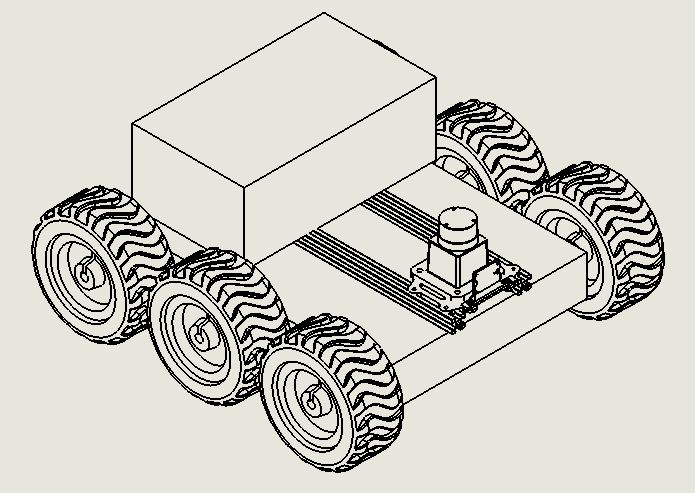
\includegraphics[width=\textwidth]{IMP}
	    \caption{Isometric view}
	    \label{fig:IMP}
    \end{subfigure}
    \quad %add desired spacing between images, e. g. ~, \quad, \qquad, \hfill etc.
      %(or a blank line to force the subfigure onto a new line)
    \begin{subfigure}[b]{0.3\textwidth}
        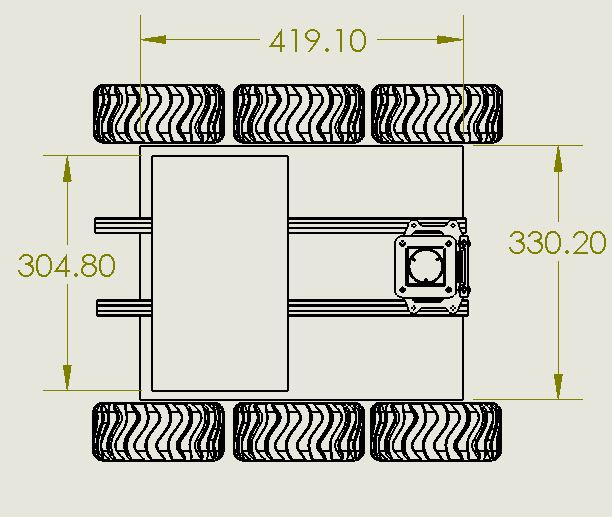
\includegraphics[width=\textwidth]{IMPtop}
        \caption{Top view}
        \label{fig:IMPtop}
    \end{subfigure}%
    \quad %add desired spacing between images, e. g. ~, \quad, \qquad, \hfill etc.
      %(or a blank line to force the subfigure onto a new line)
    \begin{subfigure}[b]{0.3\textwidth}
        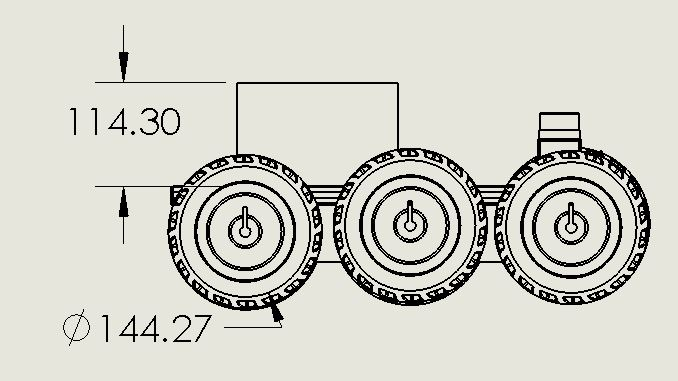
\includegraphics[width=\textwidth]{IMPside}
        \caption{Side view}
        \label{fig:IMPside}
    \end{subfigure}%
    \caption{Dimensions of \imp}
    \label{fig:IMPviews}
\end{figure}

\section{Electrical Components}
The major Electrical Components on the IMP can be classified under 4 main categories as shown in figure \ref{fig: blockDiag}. Starting with the power we use a Lithium Polymer battery supplying 12V and regulate it on the Power regulation board,component J, to 5V for the Odroid which serves as the on-board computer(Component I on the table \ref{tab: Components}). Since we are using an autopilot board, the Inertial Measurement Unit and the micro-controller are integrated in the same component A in figure \ref{fig:IMPfront}. The other sensors are distributed between the autopilot and the Odroid. The motor driver of choice is the Sabertooth 2x12 as it has a differential command mode in which velocity and omega PWMs are converted to individual motor voltages in hardware. 

\begin{figure}[h!]
    \centering
    \begin{subfigure}[b]{0.4\textwidth}
	    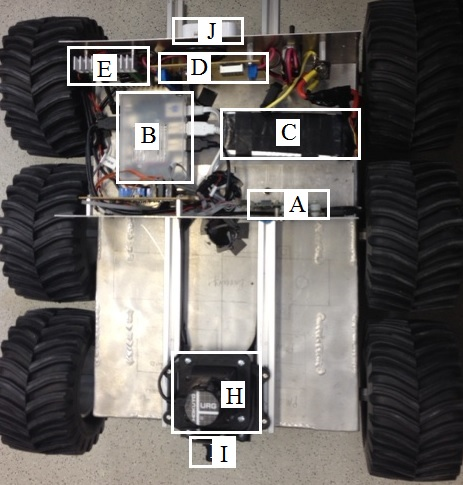
\includegraphics[width=\textwidth]{IMPfront}
	    \caption{Top view}
	    \label{fig:IMPfront}
    \end{subfigure}
    \quad %add desired spacing between images, e. g. ~, \quad, \qquad, \hfill etc.
      %(or a blank line to force the subfigure onto a new line)
    \begin{subfigure}[b]{0.3\textwidth}
		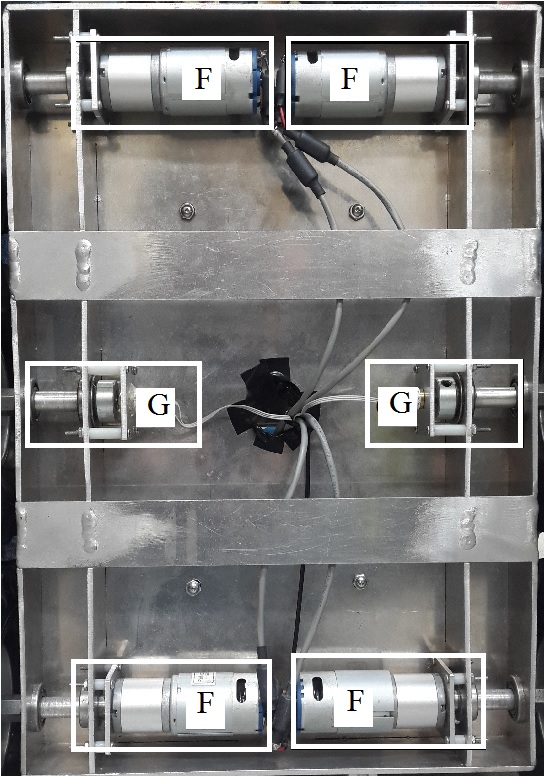
\includegraphics[width=\textwidth]{IMPback}
		\caption{Bottom view}
		\label{fig:IMPback}
    \end{subfigure}%
    \caption{Electrical components on the \imp}
    \label{fig:IMPparts}
\end{figure}

%\begin{table}[h!]
\begin{longtable}{| l | p{3cm} | p{10cm} |}
		\caption{List of major components on the IMP}
		\label{tab: Components}\\

 		\hline
 		Label & Component & Description \\ \hline 
 		\endhead
 		
 		\hline \multicolumn{3}{|r|}{{Continued on next page}} \\ \hline
 		\endfoot
 		
 		\hline \hline
 		\endlastfoot
 		
 		A & Autopilot & A multi processor control and sensing unit. 
	 		\\ & & $ \bullet $ 220 Mhz RM48L952 primary micro-controller with 256 kB internal RAM and 3MB internal Flash 
	 		\\ & & $ \bullet $ 80 Mhz TM4C123GH6PZ secondary micro-controller with 32 kB internal RAM and 256 kB internal Flash 
	 		\\ & & $ \bullet $ 10 UARTs with 2 configurable for interprocessor communication 
	 		\\ & & $ \bullet $ 12 ADC inputs 
	 		\\ & & $ \bullet $ 16 PWM outputs	
 		\\ \hline
		B & ODROID-XU3 & The on-board computer
			\\ & & $ \bullet $ Samsung Exynos5422 Cortex™-A15 2.0Ghz quad core and Cortex™-A7 quad core CPUs
	 		\\ & & $ \bullet $ 2Gbyte LPDDR3 RAM at 933MHz (14.9GB/s memory bandwidth)
	 		\\ & & $ \bullet $ USB 3.0 Host x 1, USB 3.0 OTG x 1, USB 2.0 Host x4  
 		\\ \hline
 		C & Battery & 12V Lithium Polymer battery in 3S1P configuration with 2500 mAh capacity.
 		\\ \hline
 		D & Power Board & Provide multiple connections for 12 V power along with a battery monitoring circuit. Also provide 5V regulated power for the Odroid. 
 		\\ \hline
 		E & Motor Driver & Sabertooth 2x12 regenerative dual motor driver
			\\ & & $ \bullet $ 12A continuous, 25A peak per channel
			Up to 24V in
	 		\\ & & $ \bullet $ Synchronous regenerative drive
	 		\\ & & $ \bullet $ Ultra-sonic switching frequency
	 		\\ & & $ \bullet $ Input modes: Analog, R/C, simplified serial, packetized serial
 		\\ \hline
 		F & Motors & 165 RPM HD Precision Planetary Gear Motor
 			\\ & & $ \bullet $ Rated Voltage: 12VDC
 			\\ & & $ \bullet $ Rated Load: 7.3 kgf-cm (101.4 oz-in)
 			\\ & & $ \bullet $ Max. Stall Current: 20A @ 12VDC
 		\\ \hline
 		G & Encoders & MA3 Miniature Absolute Magnetic Shaft Encoder
 			\\ & & $ \bullet $ 10-bit Analog output - 2.6 kHz sampling rate
 			\\ & & $ \bullet $ Reports the shaft position over $ 360^\circ $ with no stops or gaps
 		\\ \hline
 		H & Camera & 5M HD USB Camera
 			\\ & & $ \bullet $ USB 2.0 compliance
  			\\ & & $ \bullet $ Focusing Range: 60cm to infinity	
   			\\ & & $ \bullet $ Fov (H): 72°
 		\\ \hline
 		I & LIDAR &  Hokuyo URG-04LX-UG01 Scanning Laser Rangefinder
 			\\ & & $ \bullet $ Detectable range of 20mm to 5600mm
 			\\ & & $ \bullet $ 100msec/scan
 			\\ & & $ \bullet $ 240° area scanning range with 0.36° angular resolution
 		\\ \hline
 		J & Wifi Module & TP-LINK Nano Wireless Travel Router
 			\\ & & $ \bullet $ 150Mbps Wi-Fi speed
 			\\ & & $ \bullet $ Supports AP, Client, Router, Repeater, and Bridge modes
 			\\ & & $ \bullet $ Compatible with 802.11b/g/n and 2.4GHz Wi-Fi devices
 			 			 			 		
 		\\ \hline 
	\end{longtable}
%\end{table}

\section{Control Process}
\begin{figure}[h]
\centering
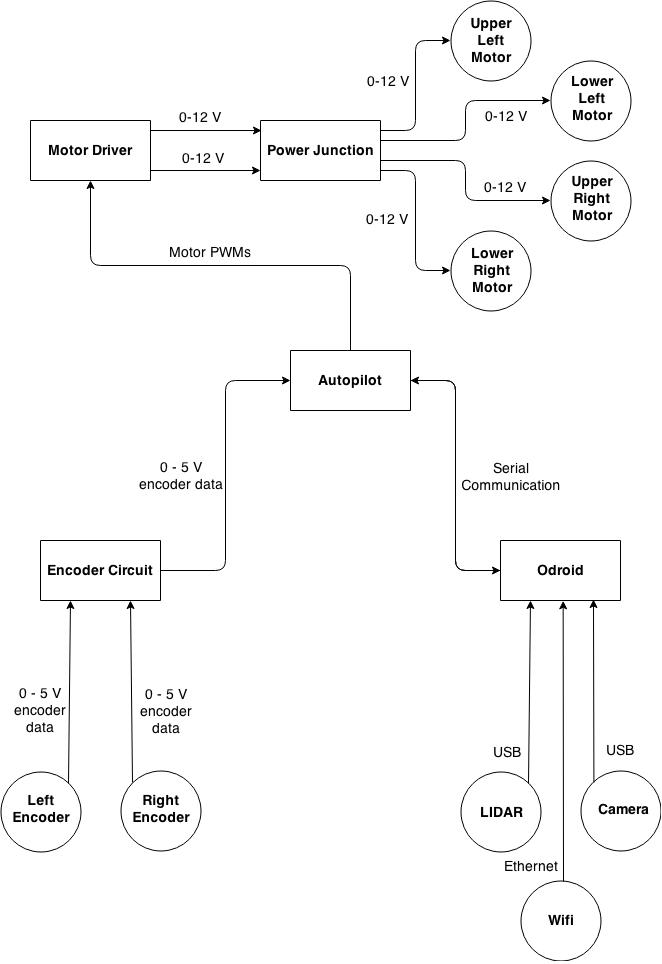
\includegraphics[width=\textwidth]{commdiag}
\caption{Communication Diagram}
\label{fig: CommDiag}
\end{figure}
Another major part of the electrical circuits is the communication and information flow between the various components. The control decisions taken are mainly based on this. Each of the components have different means and protocols of communication. The communication setup is shown in figure \ref{fig: CommDiag} Once all the communication channels are established the information flow is designed as follows.
\begin{itemize}
	\item The Autopilot maintains timebase for the whole process. It also reads in the Encoder and IMU. All this information is sent to on-board computer through the serial port. It also logs all the data on an on-board SD card.
	\item The Odroid then reads the LIDAR and Camera data at that time. It logs both the data read in and the data it received from the autopilot. 
	\item The user commands are sent to the Odroid through the Wi-Fi and are transmitted as is or after interpretation as per the algorithm and the kind of commands being sent. 
\end{itemize}

%\section{Code Structure} 
